\documentclass{article}
\usepackage[utf8]{inputenc}
\usepackage[spanish]{babel}
\usepackage{listings}
\usepackage{graphicx}
\graphicspath{ {images/} }
\usepackage{cite}
\usepackage{enumerate} % enumerados

\begin{document}

\begin{titlepage}
    \begin{center}
        \vspace*{1cm}
            
        \Huge
        \textbf{CALISTENIA}
            
        \vspace{0.5cm}
        \LARGE
        Actividad 1
            
        \vspace{1.5cm}
            
        \textbf{Juan Esteban Grisales Gallego}
            
        \vfill
            
        \vspace{0.8cm}
            
        \Large
        Despartamento de Ingeniería Electrónica y Telecomunicaciones\\
        Universidad de Antioquia\\
        Medellín\\
        Marzo de 2021
            
    \end{center}
\end{titlepage}

\tableofcontents
\newpage
\section{Sección introductoria}\label{intro}


\begin{itemize}
    \item Posición inicial: Las tarjetas juntas verticalmente recostadas sobre la        mesa   debajo de la hoja y que la hoja quede centrada respecto a las tarjetas.
    \item Siga paso a paso las instrucciones.

\end{itemize}

\section{Sección de contenido} \label{contenido}



Pasos a seguir:

\begin{enumerate}[1.]

    \item Ubícate frente a la hoja, luego tómala y ponla al lado derecho de las             tarjetas si eres diestro o al lado izquierdo si eres zurdo y que la hoja          quede sobre la mesa. ''Ten en cuenta que la tarjeta 1 es la que se ve a           simple vista y la 2 es la que está debajo’'.
    \item Si eres diestro mira el paso 3, pero si eres zurdo mira el paso 4.
    \item Con la mano derecha, teniendo en cuenta que las tarjetas están ubicadas de        forma vertical sobre la mesa; toma las dos tarjetas juntas, con el dedo           pulgar en el lado izquierdo de las tarjetas, el dedo medio en el lado             derecho y el dedo índice en el lado superior.
    \item Con la mano izquierda, teniendo en cuenta que las tarjetas están ubicadas de       forma vertical sobre la mesa; toma las dos tarjetas juntas, con el dedo            pulgar en el lado derecho de las tarjetas, el dedo medio en el lado               izquierdo
         y en dedo índice en el lado superior
    \item Llévalas hacia el centro de la hoja quedando los bordes de la parte de            debajo de las tarjetas encima de la hoja.
    \item Sosteniendo las 2 tarjetas con el dedo índice. Con el dedo pulgar y el medio       toma la tarjeta 1 en la misma posición que tenía las 2 tarjetas.
    \item Trata de separar la tarjeta 1 de la 2 pero solo el borde de abajo,                llevándola hacia atrás con el dedo pulgar y medio. 
    \item Tratando de que las tarjetas queden en equilibrio, suelta las tarjetas con        cuidado.
\end{enumerate}


\section{Inclusión de imágenes} \label{imagenes}

En la Figura (\ref{fig:posicion1}), Se presenta la posición inicial de la actividad.

\begin{figure}[h]
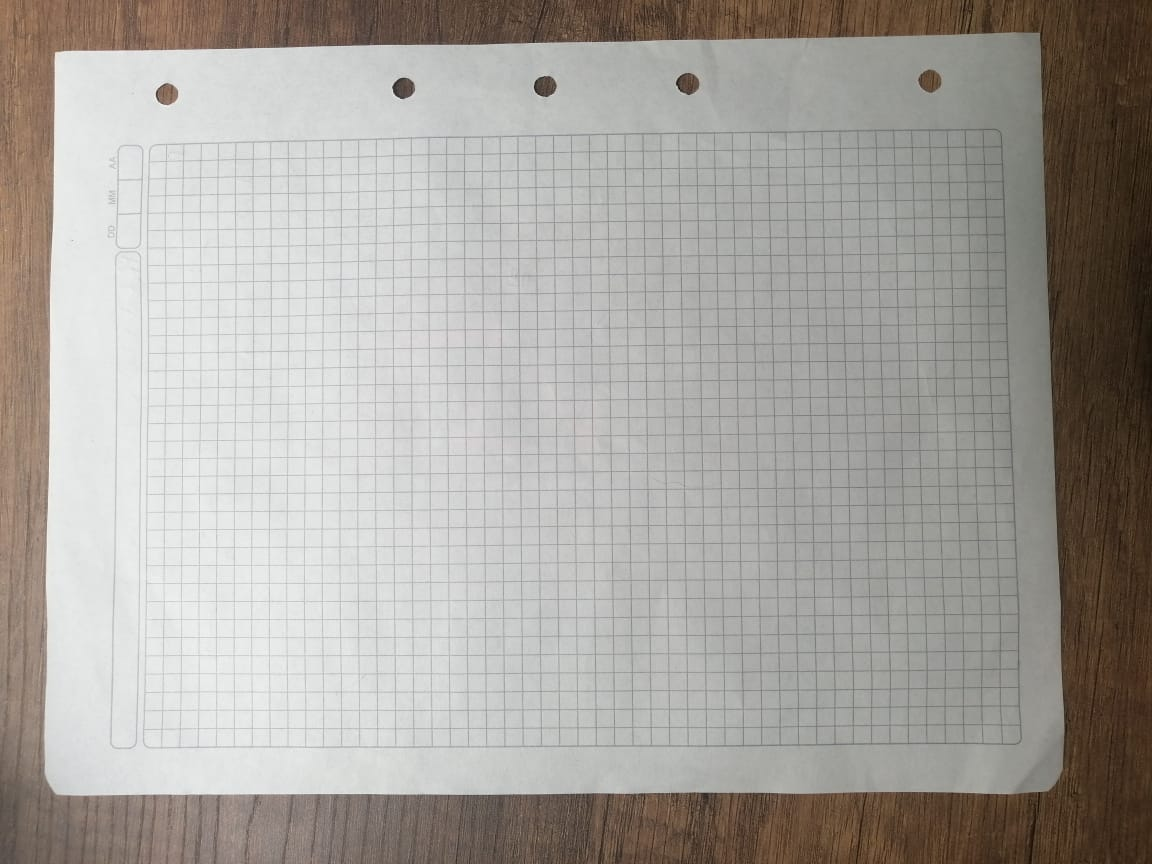
\includegraphics[width=4cm]{Posicion1.jpeg}
\centering
\caption{Posición Inicial}
\label{fig:posicion1}
\end{figure}


En la Figura (\ref{fig:posicion2}), Se presenta la posición final de la actividad.

\begin{figure}[h]
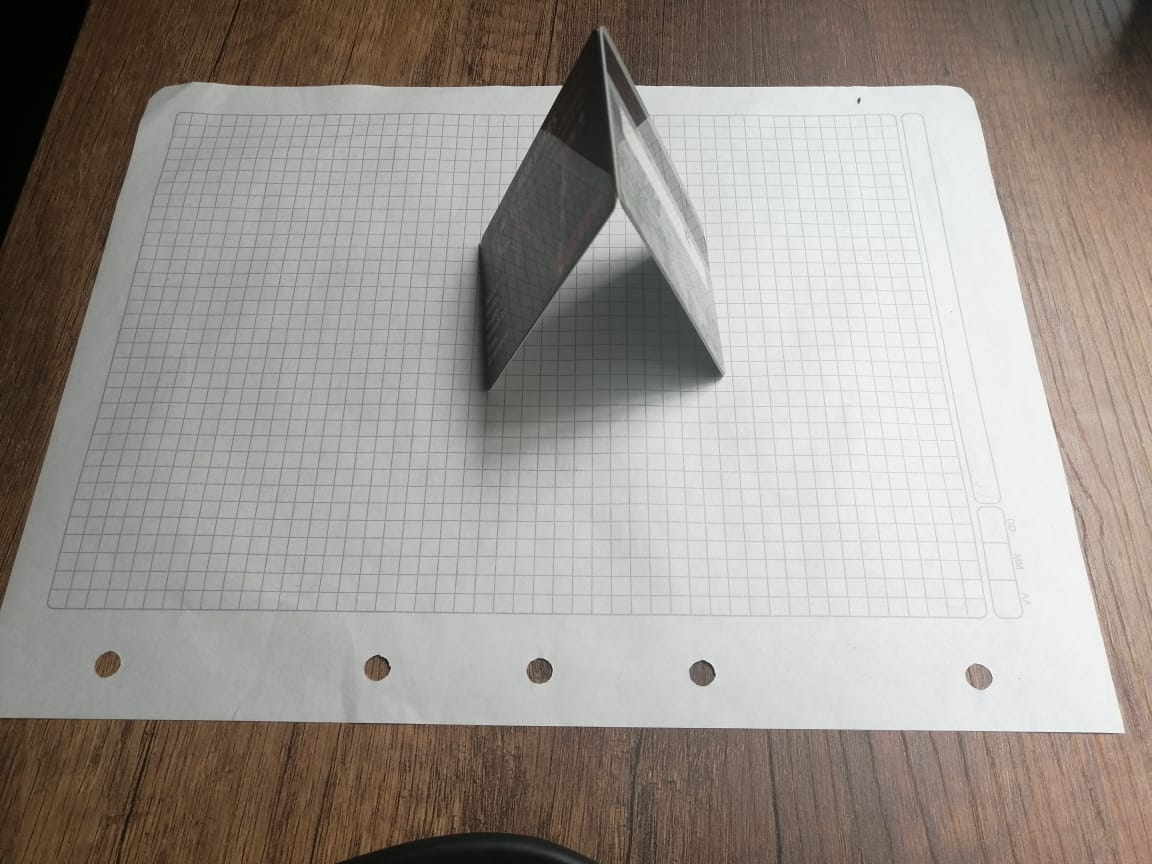
\includegraphics[width=4cm]{Posicion2.jpeg}
\centering
\caption{Posición final}
\label{fig:posicion2}
\end{figure}



\end{document}
